\begin{appendix}
\chapter{Anexo: Discretización de las Ecuaciones del BOM}\label{AnexoA}
En este apartado se presenta la discretización de las Ecuaciones del BOM \ref{ec:aceite}, \ref{ec:gas}, \ref{ec:agua} que se presentan en la subsección \ref{subsec:BOM}. Recordando:
\begin{align*}
\text{aceite: }&\frac{\partial}{\partial t} \left[ \phi \left( \frac{S_{o}}{B_{o}} + \frac{R_{v} S_{g}}{B_{g}} \right) \right]
- \nabla \cdot \left( \frac{1}{B_{o}} \vec{u_{o}} + \frac{R_{v}}{B_{g}} \vec{u_{g}} \right) - \tilde{q}_{o}=0  \\
\text{gas: }&\frac{\partial}{\partial t} \left[ \phi \left( \frac{S_{g}}{B_{g}} + \frac{R_{s} S_{o}}{B_{o}} \right) \right]
- \nabla \cdot \left( \frac{1}{B_{g}} \vec{u_{g}} + \frac{R_{s}}{B_{o}} \vec{u_{o}} \right) - \tilde{q}_{g} = 0 \\
\text{agua: }&\frac{\partial}{\partial t} \left[\phi \left( \frac{S_{w}}{B_{w}} \right) \right] - \nabla \cdot \left( \frac{1}{B_{w}} \vec{u_{w}} \right) - \tilde{q}_{w} = 0 
\end{align*}
Primero, se integran las ecuaciones sobre un intervalo de tiempo $\left[t, t+\Delta t\right]$, y una celda de control $\Omega_{i}$. Se toma como ejemplo la ecuación de conservación para el aceite \ref{ec:aceite}. Las ecuaciones para el gas y agua (\ref{ec:gas}, \ref{ec:agua}) se discretizan de manera análoga.
\begin{align*}
	\int_{t}^{t+\Delta t}\int_{\Omega_{i}}\frac{\partial}{\partial t} \left[ \phi \left( \frac{S_{o}}{B_{o}} + \frac{R_{v} S_{g}}{B_{g}} \right) \right]dVdt
	- \int_{t}^{t+\Delta t}\int_{\Omega_{i}}\nabla \cdot \left( \frac{1}{B_{o}} \vec{u_{o}} + \frac{R_{v}}{B_{g}} \vec{u_{g}} \right)dVdt \\
	- \int_{t}^{t+\Delta t}\int_{\Omega_{i}}\tilde{q}_{o}dVdt=0 
\end{align*}
Luego, se desglosan las ecuaciones en sus términos acumulativos, de flujo, y de fuentes y sumideros, debido a que cada uno de estos términos requiere un tratamiento distinto.
\begin{align*}
\underbrace{\int_{t}^{t+\Delta t}\int_{\Omega_{i}}\frac{\partial}{\partial t} \left[ \phi \left( \frac{S_{o}}{B_{o}} + \frac{R_{v} S_{g}}{B_{g}} \right) \right]dVdt}_{\text{Término de acumulación}}
- \underbrace{\int_{t}^{t+\Delta t}\int_{\Omega_{i}}\nabla \cdot \left( \frac{1}{B_{o}} \vec{u_{o}} + \frac{R_{v}}{B_{g}} \vec{u_{g}} \right)dVdt}_\text{Término de flujo} \\
- \underbrace{\int_{t}^{t+\Delta t}\int_{\Omega_{i}}\tilde{q}_{o}dVdt}_{\text{Término de fuentes y sumideros}}=0 
\end{align*}
Empezando por el término acumulativo, se sigue que, por el teorema de Fubini que
\begin{align*}
	\int_{t}^{t+\Delta t}\left(\int_{\Omega_{i}}\frac{\partial}{\partial t} \left[ \phi \left( \frac{S_{o}}{B_{o}} + \frac{R_{v} S_{g}}{B_{g}} \right) \right]dV\right)dt = \int_{\Omega_{i}}\left(\int_{t}^{t+\Delta t}\frac{\partial}{\partial t} \left[ \phi \left( \frac{S_{o}}{B_{o}} + \frac{R_{v} S_{g}}{B_{g}} \right) \right]dt\right)dV 
\end{align*}
Por teorema fundamental del cálculo
\begin{align*}
 \int_{\Omega_{i}}\left(\int_{t}^{t+\Delta t}\frac{\partial}{\partial t} \left[ \phi \left( \frac{S_{o}}{B_{o}} + \frac{R_{v} S_{g}}{B_{g}} \right) \right]dt\right)dV = \int_{\Omega_{i}}\left[ \phi \left( \frac{S_{o}}{B_{o}} + \frac{R_{v} S_{g}}{B_{g}} \right) \right]^{t+\Delta t}_{t}dV
\end{align*}
Considerando el cambio de la acumulación en un intervalo de tiempo como una constante para una celda de control $\Omega_{i}$
\begin{align*}
	\int_{\Omega_{i}}\left[ \phi \left( \frac{S_{o}}{B_{o}} + \frac{R_{v} S_{g}}{B_{g}} \right) \right]^{t+\Delta t}_{t}dV = \left[ \phi_{i} \left( \frac{S_{o,i}}{B_{o,i}} + \frac{R_{v,i} S_{g,i}}{B_{g,i}} \right) \right]^{t+\Delta t}_{t}\int_{\Omega_{i}}dV \\= |\Omega_{i}|\left[ \phi_{i} \left( \frac{S_{o,i}}{B_{o,i}} + \frac{R_{v,i} S_{g,i}}{B_{g,i}} \right) \right]^{t+\Delta t}_{t}
\end{align*}
Donde $|\Omega_{i}|$ es el volumen para una celda $i$. Continuando con la discretización del término de flujo, se discretiza primero el tiempo usando un esquema \textbf{implícito}, luego
\begin{align*}
\int_{t}^{t+\Delta t}\int_{\Omega_{i}}\nabla \cdot \left( \frac{1}{B_{o}} \vec{u_{o}} + \frac{R_{v}}{B_{g}} \vec{u_{g}} \right)dVdt = \Delta t \left[\int_{\Omega_{i}}\nabla \cdot \left( \frac{1}{B_{o}} \vec{u_{o}} + \frac{R_{v}}{B_{g}} \vec{u_{g}} \right)dV\right]^{t+\Delta t}
\end{align*}
Posteriormente, se asume que la función vectorial de velocidad $\vec{u_{f}}$ para cualquier fluido $f$ tiene derivadas de primer orden continuas. Luego, como la celda tiene una superficie cerrada, se aplica el teorema de la divergencia Gauss.
\begin{align*}
	\int_{\Omega_{i}}\nabla \cdot \left( \frac{1}{B_{o}} \vec{u_{o}} + \frac{R_{v}}{B_{g}} \vec{u_{g}} \right)dV = \int_{\partial \Omega_{i}}\left( \frac{1}{B_{o}} \vec{u_{o}} + \frac{R_{v}}{B_{g}} \vec{u_{g}} \right)\cdot \partial \vec{S_{i}}
\end{align*}
Usando celdas rectangulares, la integral sobre la frontera de una celda es la suma del término de flujo que se evalúa en cada cara, así
\begin{align*}
 \int_{\partial \Omega_{i}}\left( \frac{1}{B_{o}} \vec{u_{o}} + \frac{R_{v}}{B_{g}} \vec{u_{g}} \right)\cdot \partial \vec{S_{i}} = \sum_{c \in S_{i}}\int_{c}\left( \frac{1}{B_{o}} \vec{u_{o}} + \frac{R_{v}}{B_{g}} \vec{u}_{g} \right)\cdot \partial \vec{S_{c}}
\end{align*}
El valor del término de flujo en cada cara se aproxima usando el teorema del valor medio, luego el producto punto se evalua como el valor de la función en la cara
\begin{align*}
	\sum_{c \in S_{i}}\int_{c}\left( \frac{1}{B_{o}} \vec{u_{o}} + \frac{R_{v}}{B_{g}} \vec{u_{g}} \right)\cdot \partial \vec{S_{c}} \approx \sum_{c \in S_{i}} A_{c} \left( \frac{1}{B_{o,c}} \vec{u_{o,c}} + \frac{R_{v,c}}{B_{g,c}} \vec{u_{g,c}} \right)
\end{align*}
Aplicando las velocidades Darcy en la ecuación, se tiene
\begin{align*}
	\sum_{c \in S_{i}} A_{c} \left( \frac{1}{B_{o,c}} \vec{u_{o,c}} + \frac{R_{v,c}}{B_{g,c}} \vec{u_{g,c}} \right) \cdot \vec{n_{c}} = \sum_{c \in S_{i}} A_{c} \left( \frac{1}{B_{o,c}} \frac{\mathbb{K}_{c}k_{ro,c}}{\mu_{o,c}} \nabla \Phi_{o,c} + \frac{R_{v,c}}{B_{g,c}} \frac{\mathbb{K}_{c}k_{rg,c}}{\mu_{g,c}} \nabla \Phi_{g,c} \right)
\end{align*}
Dónde el gradiente de potencial $\nabla \Phi_{f,c}$, para cualquier fluido $f$ se aproxima como:
\begin{align*}
	\nabla \Phi_{f,c} \approx \frac{\Delta \Phi_{f,c}}{\Delta l_{c}} \approx \frac{\Phi_{f,i}-\Phi_{f,j}}{\Delta l_{c}}
\end{align*}
Donde $c$ es la cara que conecta la celda $i$ con la celda $j$, y el delta de longitud en la cara $\Delta l_{c}$ se calcula como:
\begin{align}
	\label{ec:DeltaCara}\Delta l_{c} = \frac{\Delta l_{i} + \Delta l_{j}}{2}
\end{align}
Cabe notar que, los deltas de longitud dependen de la dirección del vector normal $\vec{n}$. Por último, el término de fuentes y sumideros se aproxima de la misma manera que el termino del flujo, usando el teorema de valor medio. Así
\begin{align*}
	\int_{t}^{t+\Delta t}\int_{\Omega_{i}}\tilde{q}_{o}dVdt \approx \int_{t}^{t+\Delta t}\tilde{q}_{o,i} |\Omega_{i}|dt
	\approx \left[\tilde{q}_{o,i}\right]^{t+\Delta t} |\Omega_{i}|\Delta t
\end{align*}
tomando los tiempos $t+\Delta t$ como tiempo futuro o $n+1$ y los tiempo $t$ como tiempo pasado $n$, se obtiene la discretización de la ecuación de conservación del aceite (\ref{ec:aceiteDiscretizacion}) como:
\begin{align*}
	|\Omega_{i}|\left[ \phi_{i} \left( \frac{S_{o,i}}{B_{o,i}} + \frac{R_{v,i} S_{g,i}}{B_{g,i}} \right) \right]^{n+1}_{n} - \Delta t \sum_{c \in S_{i}} A_{c} \left[ \frac{1}{B_{o,c}} \frac{\mathbb{K}_{c}k_{ro,c}}{\mu_{o,c}} \nabla \Phi_{o,c} + \frac{R_{v,c}}{B_{g,c}} \frac{\mathbb{K}_{c}k_{rg,c}}{\mu_{g,c}} \nabla \Phi_{g,c} \right]^{n+1} \\- \left[\tilde{q}_{o,i}\right]^{n+1} |\Omega_{i}|\Delta t = 0
\end{align*}
Se define el término de transmisividad, en el cual se considera un promedio armónico que se utiliza para estimar el término $\mathbb{K}_{c}$ y se involucra la Ecuación \ref{ec:DeltaCara}, de la siguiente forma:
\begin{align*}
	&T_{o,c} = \left(\frac{2}{(\Delta l_{i}/A_{c}K_{l,i})+(\Delta l_{j}/A_{c}K_{l,j})}\right)\frac{k_{ro,c}}{\mu_{o,c}B_{o,c}}\\
	&T_{g,c} = \left(\frac{2}{(\Delta l_{i}/A_{c}K_{l,i})+(\Delta l_{j}/A_{c}K_{l,j})}\right)\frac{k_{rg,c}}{\mu_{g,c}B_{g,c}}
\end{align*}
Luego la ecuación de conservación que se discretiza queda:
\begin{align*}
|\Omega_{i}|\left[ \phi_{i} \left( \frac{S_{o,i}}{B_{o,i}} + \frac{R_{v,i} S_{g,i}}{B_{g,i}} \right) \right]^{n+1}_{n} - \Delta t \sum_{c \in S_{i}} \left[ T_{o,c} \Delta \Phi_{o,c} + R_{v,c} T_{g,c} \nabla \Phi_{g,c} \right]^{n+1} - \left[\tilde{q}_{o,i}\right]^{n+1} |\Omega_{i}|\Delta t = 0
\end{align*}

Considerando $\left[\tilde{q}_{o,i}\right]^{n+1} |\Omega_{i}|$ como un flujo volumétrico $\left[Q_{o,i}\right]^{n+1}$ e involucrando la evaluación al tiempo $n+1$ en cada uno de los términos, se tiene:
\begin{align*}
|\Omega_{i}|\left[ \phi_{i} \left( \frac{S_{o,i}}{B_{o,i}} + \frac{R_{v,i} S_{g,i}}{B_{g,i}} \right) \right]^{n+1}_{n} - \Delta t \sum_{c \in S_{i}} \left[ T_{o,c}^{n+1} \Delta \Phi_{o,c}^{n+1} + R_{v,c}^{n+1} T_{g,c}^{n+1} \Delta \Phi_{g,c}^{n+1} \right] - Q_{o,i}^{n+1} \Delta t
\end{align*}
Finalmente, dividiendo por $\Delta t$ la ecuación se obtiene:
\begin{align*}
\frac{|\Omega_{i}|}{\Delta t}\left[ \phi_{i} \left( \frac{S_{o,i}}{B_{o,i}} + \frac{R_{v,i} S_{g,i}}{B_{g,i}} \right) \right]^{n+1}_{n} - \sum_{c \in S_{i}} \left[ T_{o,c}^{n+1} \Delta \Phi_{o,c}^{n+1} + R_{v,c}^{n+1} T_{g,c}^{n+1} \Delta \Phi_{g,c}^{n+1} \right] - Q_{o,i}^{n+1} = 0
\end{align*}
La discretización de las ecuaciones de conservación para el gas y el agua (\ref{ec:gas}, \ref{ec:agua}) se obtienen de manera análoga a la del aceite.
\chapter{Anexo: Traducciones a código de la representación}
En este apartado se muestran porciones del modelo ejecutable que se programa en C++ \citep{ISO:2017:IIIa}. Se elije este lenguaje porque la \textit{Stardard Template Library} (STL) tiene facilidades que permiten hacer la consistencia del código con el esquema preconceptual explícita, tal como se muestra en la sección \ref{sec:conc++}. Se emula una base de datos a partir de arreglos globales que almacenan cada concepto, y, las claves foráneas que se generan entre conceptos se traducen como punteros. \\

A continuación se muestra, a modo de ejemplo, las traducciones de algunos conceptos, funciones, o porciones del EP a código C++ para verificar la consistencia del código con el modelo ejecutable. Primero, se definen los elementos que conforman las condiciones iniciales, y, la base de datos que se emula, es decir, los arreglos que contienen los conceptos que se instancian en la ejecución de las relaciones dinámicas del EP. Posteriormente, se muestran las traducciones a código de dos conceptos clase, ``Malla'' y ``Roca'', y la traducción de la relación dinámica ``Petrofísico caracteriza Roca''. Luego, se explica la traducción del cálculo del residual en el evento ``Presión del Fluido Varía''.\\

Las condiciones iniciales, en las que se definen variables globales y constantes, se programan en un \textit{namespace} ``Global'' que agrupa todas las definiciones, tal como aparecen en la figura \ref{fig:EjInitialConditions}. El código para las condiciones iniciales se expone en la tabla \ref{tab:InitialConditions}.\\

\begin{table}[h]
	\centering
	\begin{tabular}{cc}
		\parbox[c]{10em}{
			\begin{tabular}[c]{@{}c@{}}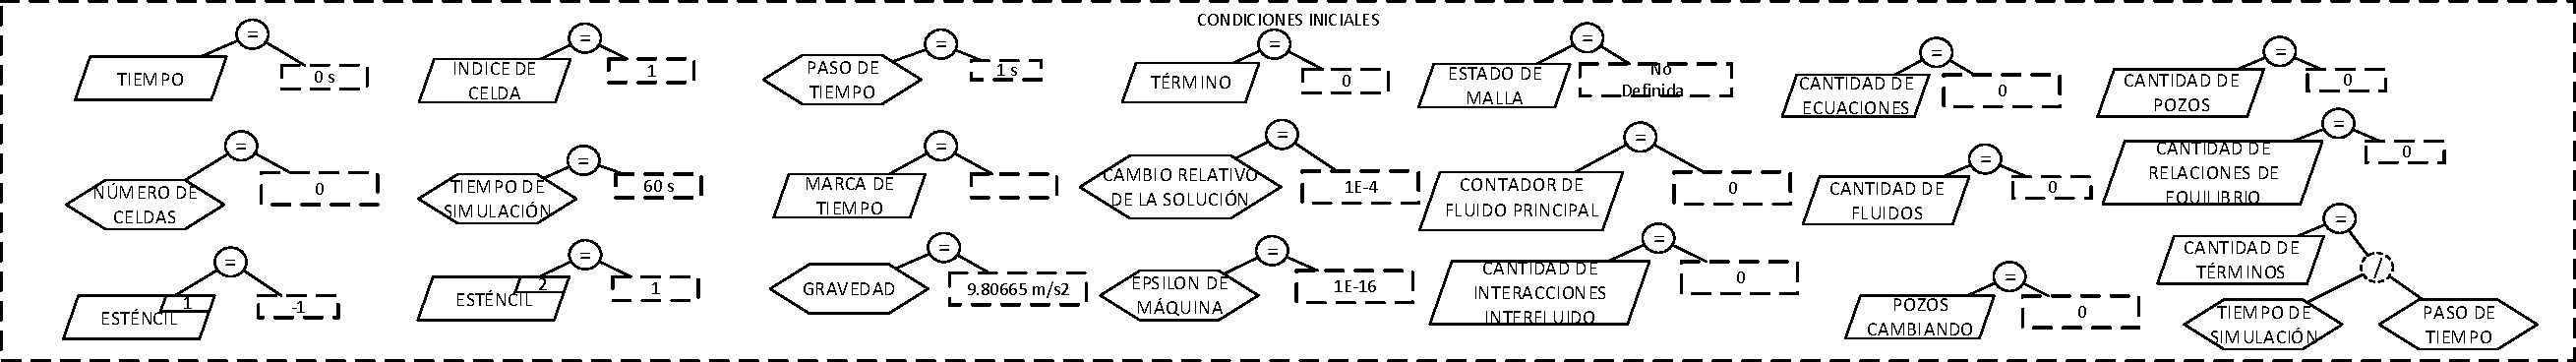
\includegraphics[width=3in]{Fig/EjInitialConditions.pdf}\\ Ver figura \ref{fig:EjInitialConditions}.\end{tabular}
			%
			%\caption[Elementos para la representación de Software Científico.]{Elementos para la representación de Software Científico. \citep{JCalle,norena2018det}.} \label{fig:RockTranslation}
		}
		&
		\begin{tiny}
			\begin{lstlisting}
			namespace Global{
			
			std::string timestamp="";
			double mytime=0;
			double simulationtime = 86400;
			double timedelta=1;
			int wells_quantity=0;
			int term=0;
			int fluids_quantity=0;
			int stencil[2] = {-1,1};
			int equilibrium_relations_quantity=0;
			int interfluid_interactions_quantity=0;
			int cells_number=0;
			int changing_wells=0;
			
			};
			
			
			\end{lstlisting}
		\end{tiny}
	\end{tabular}
	\label{tab:InitialConditions}
	\caption[Traducción a código de las condiciones iniciales.]{Traducción a código de las condiciones iniciales. Los autores.}
\end{table}

En el código \ref{tab:bd} se muestra los conceptos que se almacenan en arreglos, estos se iteran en diferentes funciones del código. Es importante notar que, en las precondiciones del EP se establece que sólo se define una única malla y sólo se caracteriza una única roca. Por tanto, en la base de datos que se emula, estos dos conceptos se acceden por medio de un puntero único. También se destaca que, todos los objetos que se instancian de los conceptos clase, se acceden a partir de punteros. Todos los punteros se fundamentan en la STL, que se encarga de hacer la respectiva gestión del uso de la memoria.\\

\begin{table}
	\begin{tabular}{c}
		\begin{tiny}
			\begin{lstlisting}
			
			std::vector<std::shared_ptr<Equation_Base>> equations =
			std::vector<std::shared_ptr<Equation_Base>>();
			
			std::vector<std::shared_ptr<Fluid>> characterized_fluids =
			std::vector<std::shared_ptr<Fluid>>();
			
			std::vector<std::unique_ptr<Equilibrium_Relation>> added_equilibrium_relations =
			std::vector<std::unique_ptr<Equilibrium_Relation>>();
			
			std::vector<std::unique_ptr<Interfluid_Interaction>> added_interfluid_interactions =
			std::vector<std::unique_ptr<Interfluid_Interaction>>();
			
			std::vector<std::shared_ptr<Well>> perforated_wells =
			std::vector<std::shared_ptr<Well>>();
			
			std::unique_ptr<Mesh> mymesh;
			std::unique_ptr<Rock> myrock;
			
			\end{lstlisting}
		\end{tiny}
	\end{tabular}
	\label{tab:bd}
	\caption[Arreglos que conforman la base de datos que se emula.]{Arreglos que conforman la base de datos que se emula. Los autores.}
\end{table}

En el código \ref{tab:MeshCode} se puede observar que, la conceptualización de la malla coincide con el código que se genera para la misma. La malla se propone como un conjunto de celdas. Adicionalmente, se tienen elementos como el espesor que dependen de la cantidad de celdas en cada dirección. Las celdas también se iteran, pero su arreglo correspondiente se almacena dentro del concepto malla, tal como se propone en la sección \ref{subsec:PS_Mesh}.\\

\begin{table}[h]
	\centering
	\begin{tabular}{cc}
		\parbox[c]{5em}{
			\begin{tabular}[c]{@{}c@{}}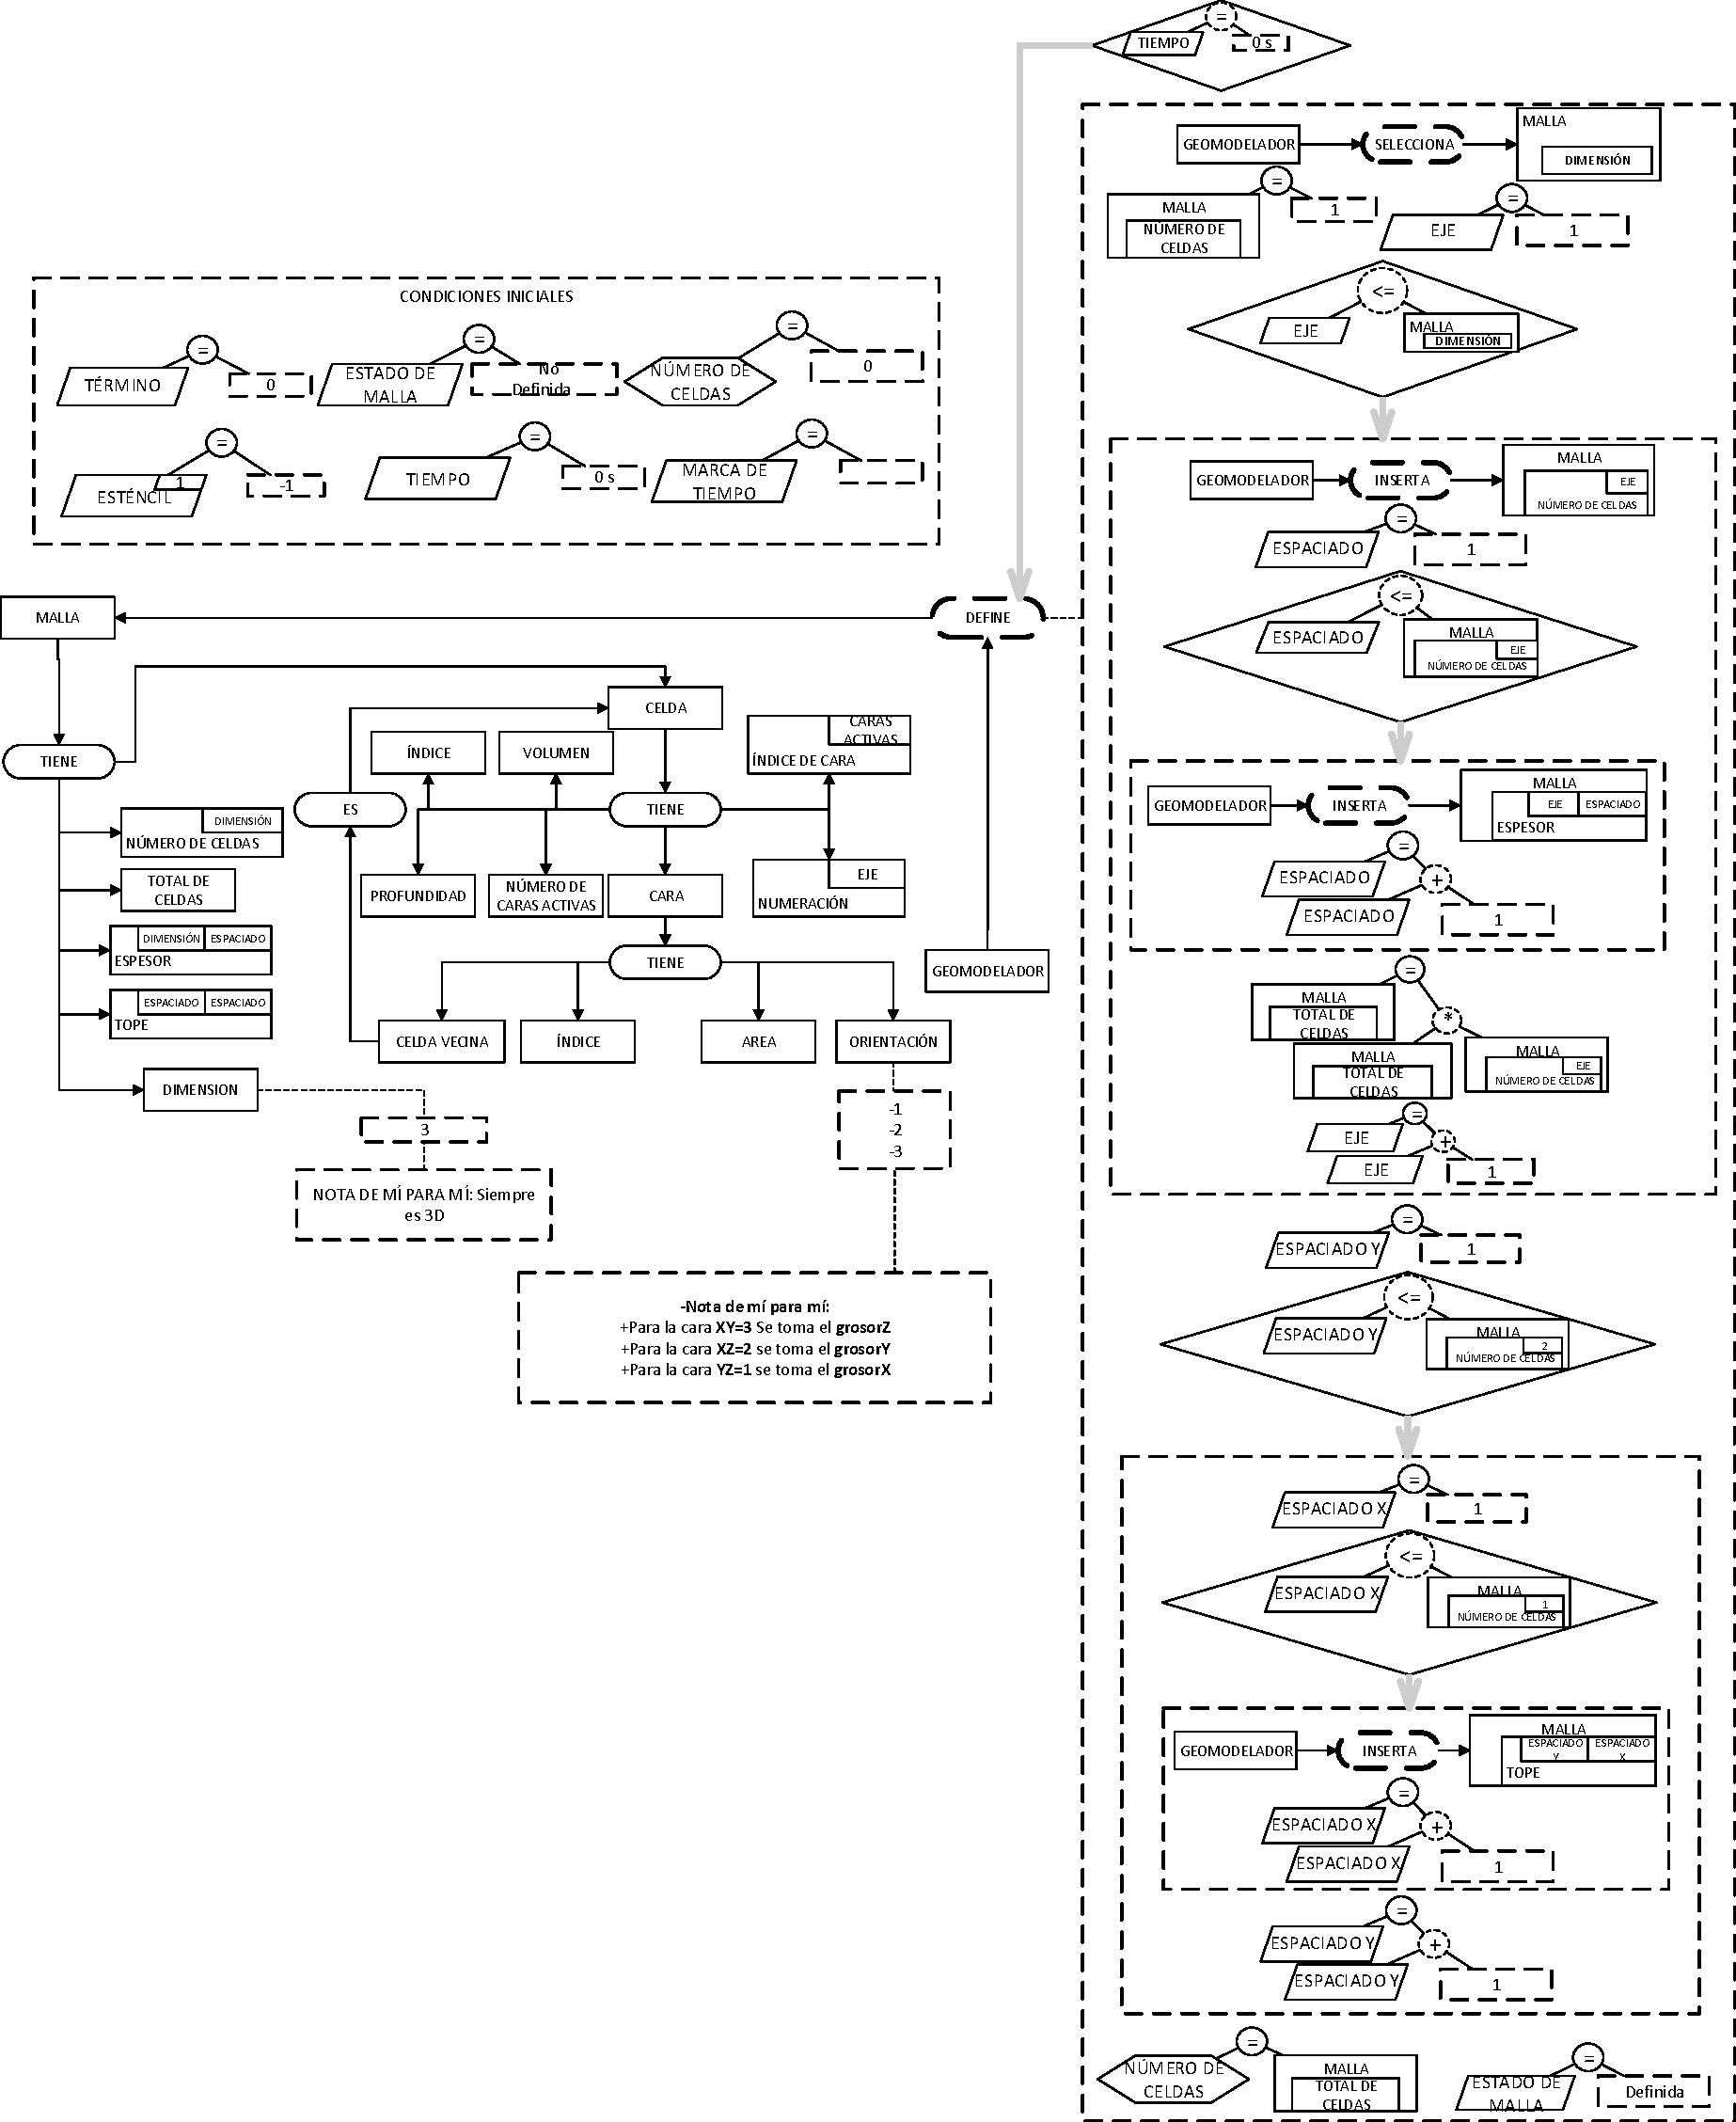
\includegraphics[width=2in]{Fig/Mesh.pdf}\\ Ver figura \ref{fig:Mesh}.\end{tabular}
			%
			%\caption[Elementos para la representación de Software Científico.]{Elementos para la representación de Software Científico. \citep{JCalle,norena2018det}.} \label{fig:RockTranslation}
		}
		&
		\begin{tiny}
			\begin{lstlisting}
			
			class Mesh{
			
			private:
			
			using Cells_t = std::vector<std::shared_ptr<Cell>>;
			int _dimension;
			std::vector<int> _cell_number = std::vector<int>(3);
			int _cell_total;
			std::vector<std::vector<double>> _thickness;
			std::vector<std::vector<double>> _top;
			int _defined=0;
			Cells_t _cells;
			
			public:
			
			using Cell_iterator = Cells_t::iterator;
			using Cell_const_iterator = Cells_t::const_iterator;
			
			Mesh();
			int getCellTotal();
			void define();
			void defineFromFile(std::ifstream& mesh_reader);
			void appear(const std::string& _timestamp, const int stencil[2]);
			
			int listCell(int posx, int posy, int posz);
			int listCell(std::vector<int> _Numeration);
			
			const std::shared_ptr<Cell>& cell(const int index) const 
			{return _cells[index];};
			
			const double& thickness(const int axis, const int spacing) const 
			{return _thickness[axis][spacing];};
			
			Cell_iterator begin() {return _cells.begin();};
			Cell_iterator end()   {return _cells.end();};
			
			Cell_const_iterator begin()  const {return _cells.begin();};
			Cell_const_iterator end()    const {return _cells.end();};
			Cell_const_iterator cbegin() const {return _cells.cbegin();};
			Cell_const_iterator cend()   const {return _cells.cend();};
			
			
			};
			
			\end{lstlisting}
		\end{tiny}
	\end{tabular}
	\label{tab:MeshCode}
	\caption[Traducción a código del concepto Malla.]{Traducción a código del concepto Malla. Los autores.}
\end{table}



\begin{table}[h]
	\centering
	\begin{tabular}{cc}
		\parbox[c]{1em}{
			\begin{tabular}[c]{@{}c@{}}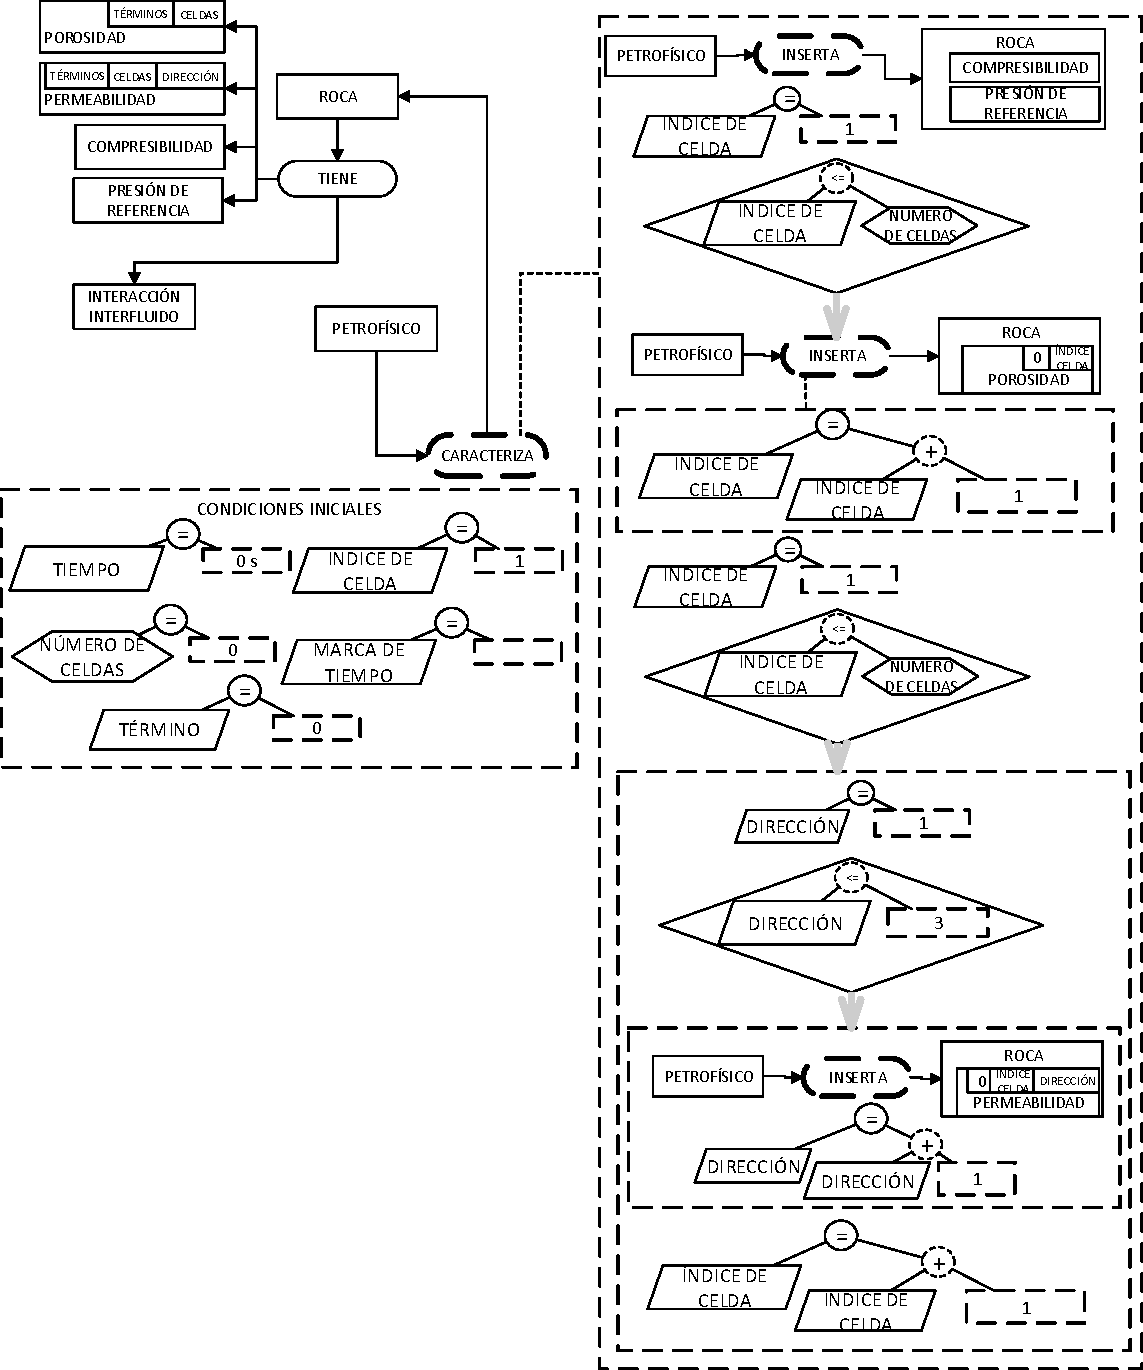
\includegraphics[width=1in]{Fig/Rock.pdf}\\ Ver figura \ref{fig:Rock}.\end{tabular}
			%
			%\caption[Elementos para la representación de Software Científico.]{Elementos para la representación de Software Científico. \citep{JCalle,norena2018det}.} \label{fig:RockTranslation}
		}
		&
		\begin{tiny}
			\begin{lstlisting}
			class Rock{
			private:
			
			double _reference_pressure;
			double _compressibility;
			std::vector<std::vector<std::vector<double>>> _absolute_permeability;   
			std::vector<std::vector<double>> _porosity;
			
			public:
			
			Rock(){};
			void characterize(const int& cells_number);
			void characterizeFromFile(std::ifstream& rock_reader,
			const int& cells_number);
			void porosity(const int term, const int cell_index,
			const double pressure);
			
			void updateProperties(const int& term);
			
			const double& porosity (const int term, const int cells_number) const {
			return _porosity[term][cells_number];
			};
			
			const std::vector<double>& absolutePermeability
			(const int term, const int cells_number) const {
			return _absolute_permeability[term][cells_number];
			};
			};
			
			\end{lstlisting}
		\end{tiny}
	\end{tabular}
	\label{tab:RockCode}
	\caption[Traducción a código del concepto Roca.]{Traducción a código del concepto Roca. Los autores.}
\end{table}

\begin{table}[h]
	\centering
	\begin{tabular}{cc}
		\parbox[c]{5em}{
			\begin{tabular}[c]{@{}c@{}}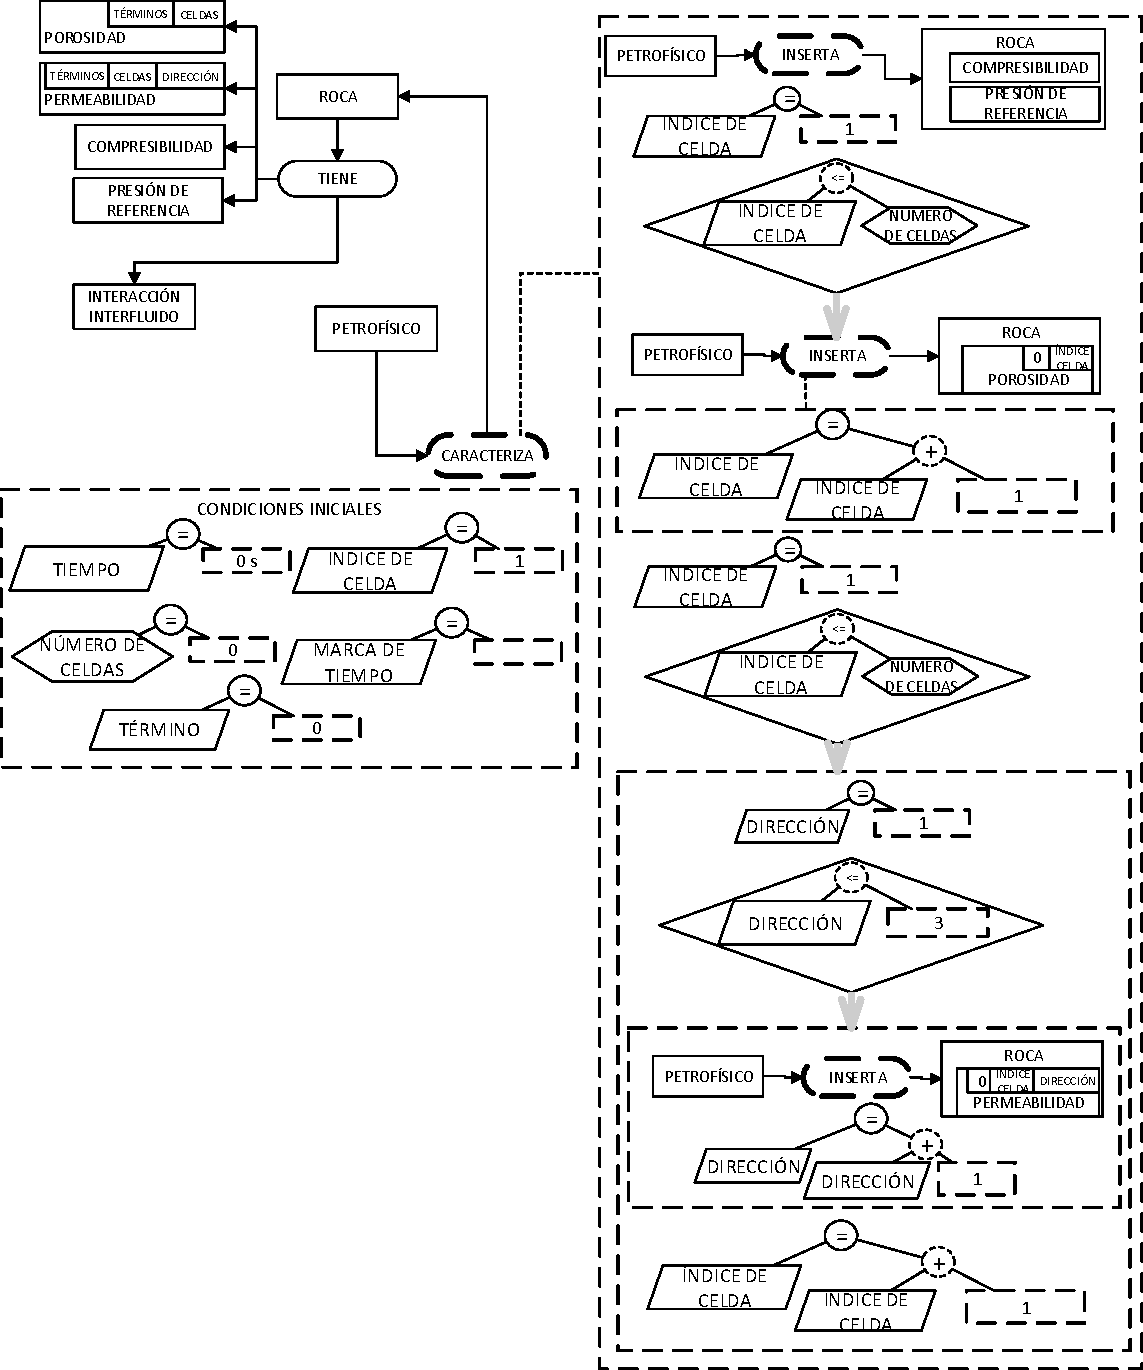
\includegraphics[width=1.5in]{Fig/Rock.pdf}\\ Ver figura \ref{fig:Rock}.\end{tabular}
			%
			%\caption[Elementos para la representación de Software Científico.]{Elementos para la representación de Software Científico. \citep{JCalle,norena2018det}.} \label{fig:RockTranslation}
		}
		&
		\begin{tiny}
			\begin{lstlisting}
			void Rock::characterize(const int& cells_number){
			
			std::ostringstream ss = std::ostringstream();
			const std::string axisnames[3]={"x", "y", "z"};
			
			_absolute_permeability = std::vector<std::vector<std::vector<double>>>
			(1,std::vector<std::vector<double>>(cells_number,std::vector<double>(3)));
			_porosity              = std::vector<std::vector<double>>(1,std::vector<double>(cells_number));
			
			myRead(std::string("Please insert rock compressibility [1/Pa]"), _compressibility,
			std::string("Please insert a valid input"));
			
			myRead(std::string("Please insert reference pressure [Pa]"), _reference_pressure,
			std::string("Please insert a valid input"));
			
			for(int cellindex=0; cellindex<cells_number; ++cellindex){
			
			ss << "Please insert initial porosity for the "<< cellindex+1 << " cell [-]";
			myRead(ss.str(), _porosity[0][cellindex], std::string("Please insert a valid input"));
			ss.str("");
			ss.clear();
			
			
			};
			for(int cellindex=0; cellindex<cells_number; ++cellindex){
			for(int direction=0; direction<3;++direction){
			ss << "Please insert initial absolute permeability for the "<< cellindex+1
			<< " cell in direction " << axisnames[direction] << " [m2]";
			myRead(ss.str(), _absolute_permeability[0][cellindex][direction],
			std::string("Please insert a valid input"));
			ss.str("");
			ss.clear();
			};
			};
			};
			
			\end{lstlisting}
		\end{tiny}
	\end{tabular}
	\label{tab:RockCharacterizeCode}
	\caption[Traducción a código de la relación dinámica ``Petrofísico caracteriza Roca''.]{Traducción a código de la relación dinámica ``Petrofísico caracteriza Roca''. Los autores.}
\end{table}

\begin{table}[h]
	\centering
	\begin{tabular}{cc}
		\parbox[c]{7em}{
			\begin{tabular}[c]{@{}c@{}}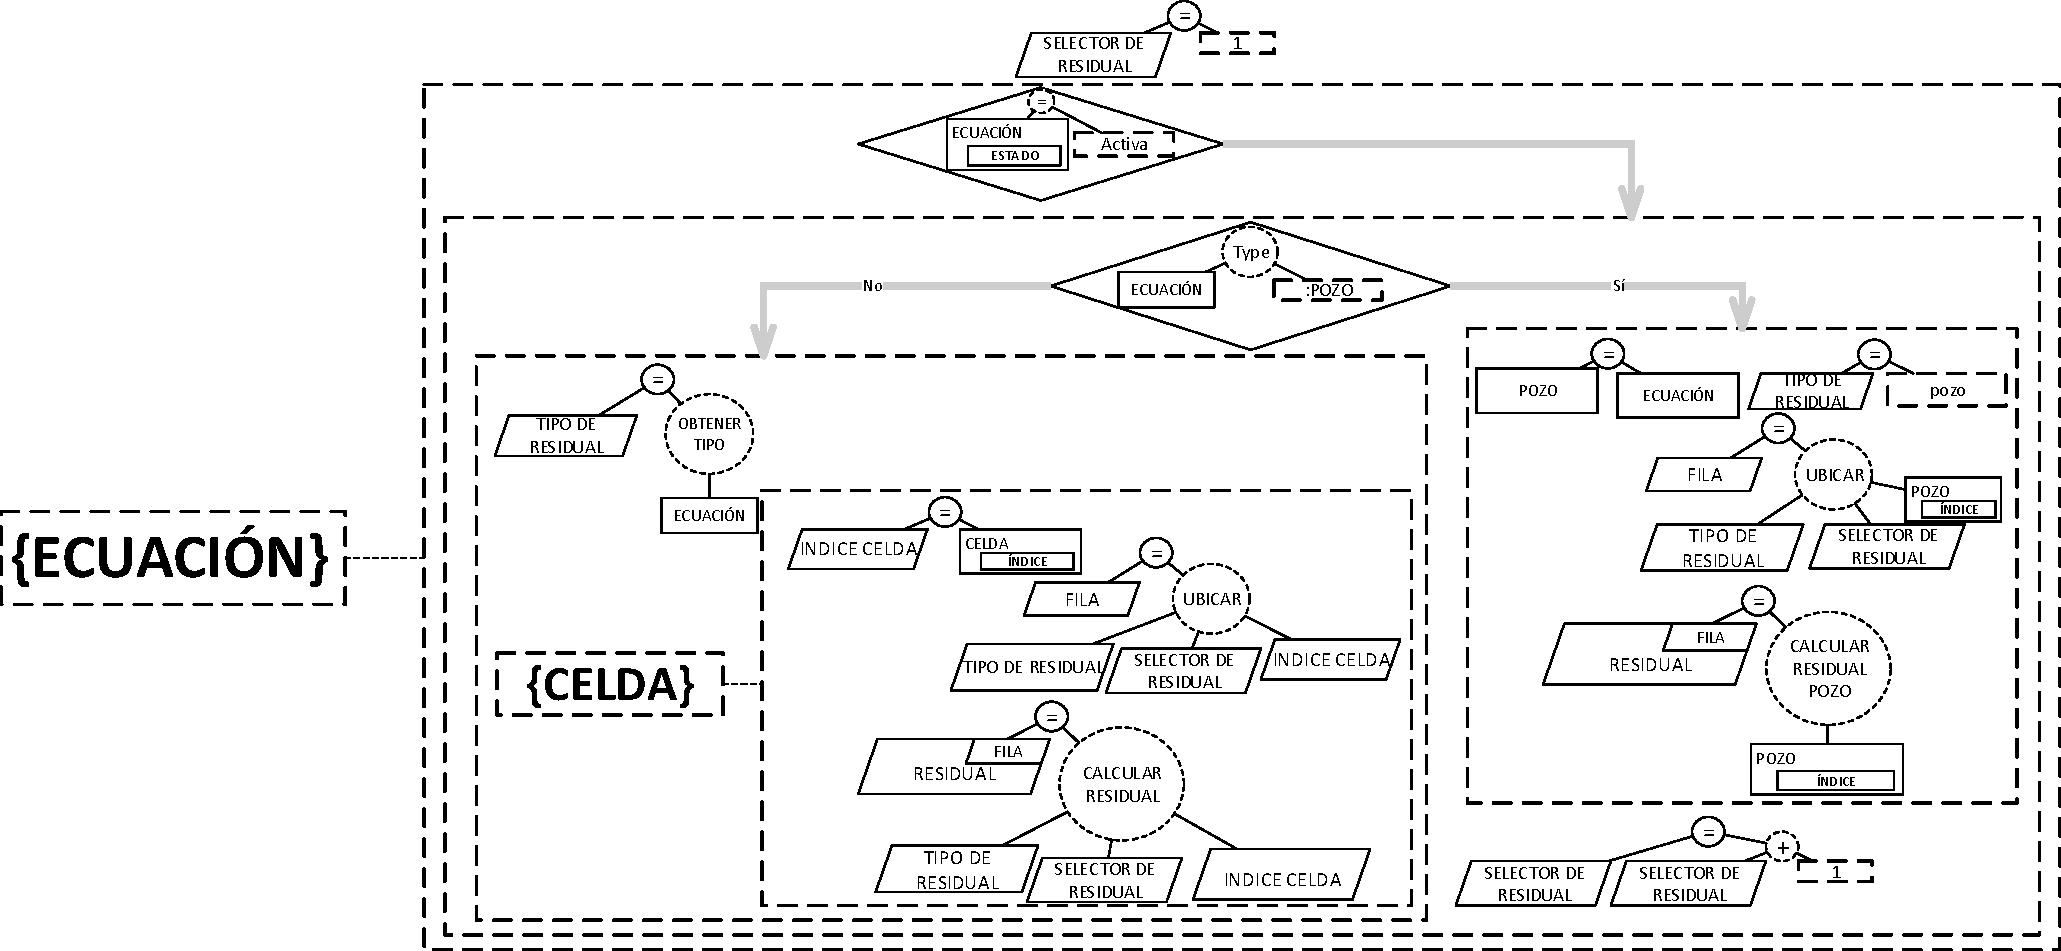
\includegraphics[width=2.5in]{Fig/Residual.pdf}\\ Ver figura \ref{fig:Residual}.\end{tabular}
			%
			%\caption[Elementos para la representación de Software Científico.]{Elementos para la representación de Software Científico. \citep{JCalle,norena2018det}.} \label{fig:RockTranslation}
		}
		&
		\begin{tiny}
			\begin{lstlisting}
			//Residual calculation
			residual_selector = 0;
			
			for(auto equation : equations){
			
			if(equation->status()){
			
			if(equation->type() == typeid(Well).name()){
			
			constexpr auto residual_type = "well";
			auto residual_well = std::dynamic_pointer_cast<Well,Equation_Base>(equation);
			
			row = locate(residual_type, residual_selector, residual_well->index());
			_residual(row) = calculateWellResidual(term, residual_well);
			
			}else{
			
			constexpr auto residual_type = "fluid";
			auto residual_fluid = std::dynamic_pointer_cast<Fluid,Equation_Base>(equation);
			
			for(auto cell = mesh.begin(); cell != mesh.end(); ++cell){
			
			cell_index = (*cell)->index();
			
			row = locate(residual_type, residual_selector, cell_index);
			
			_residual(row) = 
			calculateResidual(term,*residual_fluid, mesh, *cell, rock, wells);
			
			};
			};
			
			++residual_selector;
			
			};
			};
			
			\end{lstlisting}
		\end{tiny}
	\end{tabular}
	\label{tab:ResidualCode}
	\caption[Traducción a código del cálculo de residual en el evento ``Presión del Fluido Varía''.]{Traducción a código del cálculo de residual en el evento ``Presión del Fluido Varía''. Los autores.}
\end{table}

%\chapter{Anexo: Pirobos todos}\label{AnexoSizas}
%\newpage
%\begin{small}
%	\begin{lstlisting}
%	double calculateAccumulation
%	    (const int& term, Fluid& fluid, 
%	        const std::shared_ptr<Cell>& cell, Rock& rock){
%	
%	double past_contribution=0;
%	double current_contribution=0;
%	
%	const int cell_index = cell->index();
%	
%	for(auto& equilibrium_relation : added_equilibrium_relations ){
%	
%	if(equilibrium_relation->receiverFluid()->index() == fluid.index()){
%	
%	const auto contributor = equilibrium_relation->contributorFluid();
%	
%	double past_coef = 
%	    equilibrium_relation->partitionCoefficient(term-1,cell_index);
%	
%	past_contribution = past_contribution +
%	past_coef * (rock.porosity(term-1,cell_index) * 
%	contributor->saturation(term-1,cell_index)
%	/ contributor->volumetricFactor(term-1,cell_index));
%	
%	double curr_coef = 
%	    equilibrium_relation->partitionCoefficient(term,cell_index);
%	
%	current_contribution = current_contribution +
%	curr_coef * (rock.porosity(term,cell_index) * 
%	contributor->saturation(term,cell_index)
%	/ contributor->volumetricFactor(term,cell_index));
%	
%	};
%	};
%	
%	double accumulation = (cell->volume()/Initial_Conditions::timedelta) *
%	(((rock.porosity(term,cell_index)*fluid.saturation(term,cell_index)
%	/fluid.volumetricFactor(term,cell_index)) + current_contribution)-
%	((rock.porosity(term-1,cell_index)*fluid.saturation(term-1,cell_index)
%	/fluid.volumetricFactor(term-1,cell_index)) + past_contribution));
%	
%	return accumulation;
%	};
%	\end{lstlisting}
%\end{small}

%A final del documento es opcional incluir \'{\i}ndices o glosarios. \'{E}stos son listas detalladas y especializadas de los t\'{e}rminos, nombres, autores, temas, etc., que aparecen en el mismo. Sirven para facilitar su localizaci\'{o}n en el texto. Los \'{\i}ndices pueden ser alfab\'{e}ticos, cronol\'{o}gicos, num\'{e}ricos, anal\'{\i}ticos, entre otros. Luego de cada palabra, t\'{e}rmino, etc., se pone coma y el n\'{u}mero de la p\'{a}gina donde aparece esta informaci\'{o}n.\\

%\chapter{Anexo: Nombrar el anexo C de acuerdo con su contenido}
%MANEJO DE LA BIBLIOGRAF\'{I}A: la bibliograf\'{\i}a es la relaci\'{o}n de las fuentes documentales consultadas por el investigador para sustentar sus trabajos. Su inclusi\'{o}n es obligatoria en todo trabajo de investigaci\'{o}n. Cada referencia bibliogr\'{a}fica se inicia contra el margen izquierdo.\\
%
%La NTC 5613 establece los requisitos para la presentaci\'{o}n de referencias bibliogr\'{a}ficas citas y notas de pie de p\'{a}gina. Sin embargo, se tiene la libertad de usar cualquier norma bibliogr\'{a}fica de acuerdo con lo acostumbrado por cada disciplina del conocimiento. En esta medida es necesario que la norma seleccionada se aplique con rigurosidad.\\
%
%Es necesario tener en cuenta que la norma ISO 690:1987 (en Espa\~{n}a, UNE 50-104-94) es el marco internacional que da las pautas m\'{\i}nimas para las citas bibliogr\'{a}ficas de documentos impresos y publicados. A continuaci\'{o}n se lista algunas instituciones que brindan par\'{a}metros para el manejo de las referencias bibliogr\'{a}ficas:\\
%
%\begin{center}
%\centering%
%\begin{tabular}{|p {7.5 cm}|p {7.5 cm}|}\hline
%\arr{Instituci\'{o}n}&Disciplina de aplicaci\'{o}n\\\hline%
%Modern Language Association (MLA)&Literatura, artes y humanidades\\\hline%
%American Psychological Association (APA)&Ambito de la salud (psicolog\'{\i}a, medicina) y en general en todas las ciencias sociales\\\hline
%Universidad de Chicago/Turabian &Periodismo, historia y humanidades.\\\hline
%AMA (Asociaci\'{o}n M\'{e}dica de los Estados Unidos)&Ambito de la salud (psicolog\'{\i}a, medicina)\\\hline
%Vancouver &Todas las disciplinas\\\hline
%Council of Science Editors (CSE)&En la actualidad abarca diversas ciencias\\\hline
%National Library of Medicine (NLM) (Biblioteca Nacional de Medicina)&En el \'{a}mbito m\'{e}dico y, por extensi\'{o}n, en ciencias.\\\hline
%Harvard System of Referencing Guide &Todas las disciplinas\\\hline
%JabRef y KBibTeX &Todas las disciplinas\\\hline
%\end{tabular}
%\end{center}
%
%Para incluir las referencias dentro del texto y realizar lista de la bibliograf\'{\i}a en la respectiva secci\'{o}n, puede utilizar las herramientas que Latex suministra o, revisar el instructivo desarrollado por el Sistema de Bibliotecas de la Universidad Nacional de Colombia\footnote{Ver: www.sinab.unal.edu.co}, disponible en la secci\'{o}n "Servicios", opci\'{o}n "Tr\'{a}mites" y enlace "Entrega de tesis".

%\chapter{Sizas Tikz}
%{\color{red} \LARGE Ojo! Esto no es un anexo, es solo para pruebas}
%\begin{figure}[h!]
%	\begin{tikzpicture}
%	\begin{axis}[
%	title={Presión por Bloque},
%	xlabel={Bloque},
%	ylabel={Presión (psi)},
%	xmin=0, xmax=6,
%	ymin=1500, ymax=1550,
%	legend pos=outer north east ,
%	ymajorgrids=true,
%	xmajorgrids=true,
%	%semilogxaxis=true,
%	grid style=dashed,
%	]
%	
%	\addplot[color=blue]
%	coordinates{
%		(1,	1526.960064 )
%		(2,	1522.7829696)
%		(3,	1517.169999)
%		(4,	1512.6593172)
%		(5,	1513.1959578)
%	};
%	\addlegendentry{5 días. Autor.}
%	
%	\addplot[color=green]
%	coordinates{
%		(1,	1509.9326028)
%		(2,	1508.4097038)
%		(3,	1506.3356604)
%		(4,	1504.6822272)
%		(5,	1504.8852804)
%	};
%	\addlegendentry{10 días. Autor.}
%	
%	\addplot[color=black]
%	coordinates{
%		(1,	1503.6524574)
%		(2,	1503.101313)
%		(3,	1502.3326116)
%		(4,	1501.723452)
%		(5,	1501.795971)
%	};
%	\addlegendentry{15 días. Autor.}
%	
%	\addplot[color=purple]
%	coordinates{
%		(1,	1501.3463532)
%		(2,	1501.1433)
%		(3,	1500.853224)
%		(4,	1500.635667)
%		(5,	1500.6501708)
%	};
%	\addlegendentry{20 días. Autor.}
%	
%	\addplot[color=pink]
%	coordinates{
%		(1,	1500.490629)
%		(2,	1500.41811)
%		(3,	1500.3165834)
%		(4,	1500.2295606)
%		(5,	1500.2295606)
%	};
%	\addlegendentry{25 días. Autor.}
%	
%	
%	\addplot[]
%	coordinates{
%		(1,	1500.1715454)
%		(2,	1500.1425378)
%		(3,	1500.1135302)
%		(4,	1500.0845226)
%		(5,	1500.0845226)
%	};
%	\addlegendentry{30 días. Autor.}
%	
%	\addplot[color=orange]
%	coordinates{
%		(1,	1500.055515)
%		(2,	1500.0410112)
%		(3,	1500.0265074)
%		(4,	1500.0265074)
%		(5,	1500.0265074)
%	};
%	\addlegendentry{35 días. Autor.}
%	
%	
%	\addplot[red]
%	coordinates{
%		(1,	1500.0120036)
%		(2,	1500.0120036)
%		(3,	1500.0120036)
%		(4,	1499.9974998)
%		(5,	1499.9974998)
%	};
%	\addlegendentry{40 días. Autor.}
%	
%	
%	\addplot[only marks]
%	coordinates{
%		(1,	1524.61)
%		(2,	1520)
%		(3,	1514)
%		(4,	1509 )
%		(5,	1510)
%		
%	};
%	\addlegendentry{5 días. }
%	
%	\addplot[only marks]
%	coordinates{
%		(1,	1510.35)
%		(2,	1508.46)
%		(3,	1505.91)
%		(4,	1503.88)
%		(5,	1504.09)
%		
%	};
%	\addlegendentry{10 días.}
%	
%	\addplot[only marks]
%	coordinates{
%		(1,	1504.34)
%		(2,	1503.54)
%		(3,	1502.47)
%		(4,	1501.61)
%		(5,	1501.7)
%	};
%	\addlegendentry{15 días. }
%	
%	\addplot[only marks]
%	coordinates{
%		(1,	1501.82)
%		(2,	1501.48)
%		(3,	1501.03)
%		(4,	1500.68)
%		(5,	1500.71)
%	};
%	\addlegendentry{20 días.}
%	
%	\addplot[only marks]
%	coordinates{
%		(1,	1500.76)
%		(2,	1500.62)
%		(3,	1500.43)
%		(4,	1500.28)
%		(5,	1500.3)
%	};
%	\addlegendentry{25 días.}
%	
%	
%	\addplot[only marks]
%	coordinates{
%		(1,	1500.32)
%		(2,	1500.26)
%		(3,	1500.18)
%		(4,	1500.12)
%		(5,	1500.12)
%	};
%	\addlegendentry{30 días.}
%	
%	\addplot[only marks]
%	coordinates{
%		(1,	1500.13)
%		(2,	1500.11)
%		(3,	1500.08)
%		(4,	1500.05)
%		(5,	1500.05)
%	};
%	\addlegendentry{35 días.}
%	
%	
%	\addplot[only marks]
%	coordinates{
%		(1	,1500.06)
%		(2	,1500.05)
%		(3	,1500.03)
%		(4	,1500.02)
%		(5	,1500.02)
%	};
%	\addlegendentry{40 días.}
%	
%	\end{axis}
%	\end{tikzpicture}
%	\caption{Comparativo datos simulados contra caso de estudio de \cite{jamal2006petroleum}.}
%	\label{cora}
%\end{figure}{}
%
%
%\begin{figure}[h!]
%	\begin{tikzpicture}
%	\begin{axis}[
%	title={Datos simulados por el Autor contra caso de estudio.},
%	xlabel={Bloque},
%	ylabel={Presión (psi)},
%	xmin=0, xmax=6,
%	ymin=1500, ymax=3000,
%	legend pos=outer north east ,
%	ymajorgrids=true,
%	xmajorgrids=true,
%	%semilogxaxis=true,
%	grid style=dashed,
%	]
%	
%	\addplot[]
%	coordinates{
%		(1,2933.8141602)	
%		(2,2923.5889812)	
%		(3,2908.882128)	
%		(4,2896.698936)	
%		(5,2899.4836656)
%		
%	};
%	\addlegendentry{5 días.}
%	
%	\addplot[]
%	coordinates{
%		(1,2605.9267536)	
%		(2,2595.745086)	
%		(3,2581.1107518)	
%		(4,2569.0000788)	
%		(5,2571.741297)
%		
%	};
%	\addlegendentry{25 días.}
%	
%	\addplot[]
%	coordinates{
%		(1,2203.1127162)	
%		(2,2193.0180714)	
%		(3,2178.5287752)	
%		(4,2166.5196288)	
%		(5,2169.2463432)
%		
%	};
%	\addlegendentry{50 días.}
%	
%	\addplot[]
%	coordinates{
%		(1,1729.7812032)	
%		(2,1719.8025888)	
%		(3,1705.4728344)	
%		(4,1693.6087260)
%		(5,1696.3064328)
%		
%	};
%	\addlegendentry{80 días.}
%	\end{axis}
%	\end{tikzpicture}
%	\caption{gg izi}
%	\label{siiiizas}
%\end{figure}{}
%
%\begin{figure}[h!]
%	\begin{tikzpicture}
%	\begin{axis}[
%	title={Datos simulados por el Autor contra caso de estudio.},
%	xlabel={Bloque},
%	ylabel={Presión (psi)},
%	xmin=0, xmax=6,
%	ymin=1500, ymax=3000,
%	legend pos=outer north east ,
%	ymajorgrids=true,
%	xmajorgrids=true,
%	%semilogxaxis=true,
%	grid style=dashed,
%	]
%	
%	\addplot[]
%	coordinates{
%		(1,2933.8141602)
%		(2,2923.5889812)
%		(3,2908.882128)
%		(4,2896.698936)
%		(5,2899.4836656)
%		
%	};
%	\addlegendentry{5 días.}
%	
%	\addplot[]
%	coordinates{
%		(1,2605.9267536)
%		(2,2595.745086)
%		(3,2581.1107518)
%		(4,2569.0000788)
%		(5,2571.741297)
%		
%	};
%	\addlegendentry{25 días.}
%	
%	\addplot[]
%	coordinates{
%		(1,2203.1127162)
%		(2,2193.0180714)
%		(3,2178.5287752)
%		(4,2166.5196288)
%		(5,2169.2463432)
%		
%	};
%	\addlegendentry{50 días.}
%	
%	\addplot[]
%	coordinates{
%		(1,1729.7812032)
%		(2,1719.8025888)
%		(3,1705.4728344)
%		(4,1693.6087260)
%		(5,1696.3064328)
%	};
%	\addlegendentry{80 días.}
%	
%	\addplot[only marks]
%	coordinates{
%		(1,2936.80)
%		(2,2928.38)
%		(3,2915.68)
%		(4,2904.88)
%		(5,2908.18)
%		
%		
%	};
%	\addlegendentry{días, reportado.}
%	\addplot[only marks]
%	coordinates{
%		(1,2630.34)
%		(2,2620.06)
%		(3,2605.28)
%		(4,2593.04)
%		(5,2595.81)
%		
%		
%	};
%	\addlegendentry{días, reportado.}
%	\addplot[only marks]
%	coordinates{
%		(1,2243.97)
%		(2,2233.68)
%		(3,2218.9)
%		(4,2206.66)
%		(5,2209.43)
%		
%		
%	};
%	\addlegendentry{días, reportado.}
%	\addplot[only marks]
%	coordinates{
%		
%		(1,1780.3100)
%		(2,1770.0200)
%		(3,1755.2400)
%		(4,1743.0000)
%		(5,1745.7700)
%		
%		
%	};
%	\addlegendentry{días, reportado.}
%	\end{axis}
%	\end{tikzpicture}
%	\caption{gg}
%	\label{recora}
%\end{figure}{}

\end{appendix}